\documentclass[12pt]{template}
\usepackage{fancyhdr}
\usepackage{pdfpages}
\usepackage{titlesec}  
\usepackage{titletoc}  
% \usepackage{tocloft}
% \setCJKfamilyfont{SONG}{Adobe Fangsong Std}
\newcommand{\SONG}{\CJKfamily{SONG}}
\renewcommand{\contentsname}{目~~录} 
\makeatletter
\renewcommand \dotfill {\leavevmode \cleaders \hb@xt@ .25em{\hss .\hss }\hfill \kern \z@}
\makeatother
\titlecontents{section}[0em]{}{\thecontentslabel\quad}{}{\dotfill\contentspage[{\makebox[0pt][r]{\thecontentspage}}]}
\titlecontents{subsection}[1.5em]{}{\thecontentslabel\quad}{}{\dotfill\contentspage[{\makebox[0pt][r]{\thecontentspage}}]}
\titlecontents{subsubsection}[3.8em]{}{\thecontentslabel\quad}{}{\dotfill\contentspage[{\makebox[0pt][r]{\thecontentspage}}]}
\makeatletter
\def\@dotsep{0}
\makeatother
\setlength{\bibsep}{0pt}

\renewcommand{\bibsection}{\xjrefsection{参考文献}\fontsize{10pt}{9.5pt}\selectfont}
\begin{document} 
\includepdf[pages=-]{preface-0.pdf}
\includepdf[pages=-]{review-0.pdf}
\includepdf[pages=-]{review-0.pdf}
\pagenumbering{Roman}
\setcounter{page}{5}
% \documentclass[12pt]{template}
% \begin{document}

\begin{myparindent}{0pt}
    \textbf{论文题目:面向EBSN网络的事件预测与评价 }\\
    \textbf{学生姓名:张晓云}\\
    \textbf{指导教师:孙鹤立}
\end{myparindent}
\section*{摘\quad 要\markboth{摘\quad 要}{}}

作为直到2014年才被提出的模型,EBSN网络获得的关注度正在逐年提升。事件,作为EBSN网络的节点之一,在EBSN网络中占有举足轻重的地位。而理解事件描述对事件参与度的影响,对预测事件参与人数,设计事件推荐和事件安排系统,有重大的意义。本文着重研究了事件描述与事件参与度的关系,并比较了不同的文本处理方式对事件结果预测的影响。最后,本文尝试在原有事件描述的基础上,生成新的事件描述。

本文首先给出了事件结果预测问题的定义,使用最基本的文本处理方式——拉索回归,来处理事件描述属性,并将其用在了事件预测模型上。实验证明,在加入事件描述以及平衡了数据集以后,本文提出的模型对事件结果的预测能达到百分之八十的准确率。并且本文在原有模型的基础上,通过建立线性混合模型,并比较事件描述的确定系数的变化,定量的衡量了事件描述在事件参与度及决定事件结果中的作用。本文又在原有的事件描述处理方式的基础上,重新设计了带卷积层的神经网络和带GRU的神经网络用来处理事件描述,并使用实验证明带GRU的神经网络能够将预测的准确率提升接近3个百分点。最后本文着重考察了文本生成模型在自动撰写事件描述上的运用,本文提出了GAN\_PG,一个使用了变分自编码器作为生成模型,GRU作为判别模型的生成对抗网络,并通过它来生成事件描述。本文使用了BLEU值来衡量GAN\_PG生成的事件描述和真实事件描述的差异。经过训练后,GAN\_PG所生成的事件描述的BLEU-4值达到了0.67,充分证明了其和真实事件描述的相似性。
\\
\\
\begin{myparindent}{0pt}
    \small\textbf{关\ 键\ 词:EBSN;事件结果预测;自然语言处理;变分自编码器;生成对抗网络 }
\end{myparindent}
\newpage
\begin{myparindent}{0pt}
    \textbf{Title:Prediction and evaluation towards the event participation  of EBSN}\\
    \textbf{Name:\qquad\quad Zhang Xiaoyun}\\
    \textbf{Supervisor:\, Sun Heli}
\end{myparindent}
\section*{ABSTRACT\markboth{ABSTRACT}{}}

\begin{myparindent}{0pt}
As a model that was not introduced until 2014, the degree of attention gained by the EBSN network is increasing year by year. Event, as one of the node of the EBSN network, plays a significant role in the EBSN network. Understanding the impact of event descriptions on event participation has significant implications for predicting the number of event participants, designing event recommendation and event arrangement system. This paper's main contribution focuses on studying the relationship between event description and event participation, comparing the pros and cons of different text processing methods when applying to event participation prediction, and trying to generate new event description based on original ones, the last of which, based on the best of our knowledge, is the first attempt in this area.
\\
\\
The structure of this paper can be divided into three chapters. In the first chapter, the problem definition of event participation is given, and the most basic text processing method is used to predict the event participation. Experiments have shown that after adding event descriptions and balancing data set, our model can achieve an accuracy of 80 percent. In Chapter 2, we design two kinds of predictor, neural networks with convolutional layers and neural networks with GRUs, to deal with event prediction. Experiments show that neural networks with GRUs can improve prediction accuracy by two percentage points, which proves the power of new predictor. In chapter 3, we focus on the use of text generation models to automatically write event descriptions. We use a variational auto-encoder and GAN to generate the expected event description, and compare it with the description of real events.
\\
\\
\textbf{KEY WORDS}: EBSN; Event participation prediction; NLP; VAE; GAN 
\end{myparindent}
% \end{document}
\newpage

\vspace*{-1\baselineskip}
\tableofcontents
\newpage
\pagenumbering{arabic}
\setcounter{page}{1}

\documentclass[12pt]{template}
\usepackage{fancyhdr}

\begin{document}
\section{绪论} 
\par{
    在2014年前后,\textbf{Liu} 等学者提出了一个新的社交网络模型:\textit{EBSN}\cite{EBSN_linking},
在这篇论文中,\textbf{Liu.} 等把 \textit{EBSN} 分为线上和线下两部分,人们可以通过网络在线上互相交流,
但也可以通过参与线下活动的方式进行线下交流。这种新型的社交网络结构有很多有趣的性质,比如在事件的参与人数,组的
规模及其他层面上的长尾分布,以及较之于其他传统线上社交网络上的更为强烈的局部相关性。
}

\par{
    由于以上原因,越来越多的学者开始关注该领域,并大致分出了几个子方向:事件推荐,事件安排和其他。事件推荐更多
    的是从事件参与者的角度去考虑的,从事件参与者的兴趣标签出发,使用协同过滤,多标签聚类,随机游走或者其他的一些
    算法,来最大化某一个目标函数。由于网络规模等一些原因,获得全局最优一般是不现实的,因此相关的论文更多的是采用
    某些近似算法,来达到局部最优\cite{EBSN_event_reco}\cite{EBSN_on_social}\cite{EBSN_event_recom2}。
    事件安排的目的则是通过合理的安排每个事件的参与人员,在确保事件符合事件参与者的兴趣的同时,保证每个事件都符合
    组织者的预期:例如有足够的人参加。较之与事件推荐的不同,是事件安排同时要考虑两方面的因素,限制条件更多,例如
    活动参与人的限制,活动举办时间的限制和地点的限制,所以如何平衡好这方面的矛盾是解决这类问题的关键之一\cite{EBSN_conflict-aware_2016}
    \cite{EBSN_feedback-aware_2017}\cite{EBSN_conflict-aware_2015}。同样,想在这类问题上获得全局最优解也是很困难的,因此通过近
    似算法来得到局部最优解也是普遍的选择。
}
\par{
    除了以上两个方向,近年来关于EBSN的其他方向的研究也渐渐兴起。其中比较有趣的话题是通过研究\textit{EBSN}中人
    们如何选择和参与事件来帮助解释人群行为\cite{EBSN_understanding},以及研究话题模型在\textit{EBSN}中的传播
    方式。在\cite{EBSN_can_i}这篇论文中,由于普遍来说一个兴趣小组的三月存活率不到百分之30,因此作者通过研究组的创办者,组成员数量的增长速度以及其他因素,来预测最终该
    组是否能够存活。在\cite{EBSN_who_will}这篇论文中,作者把角度放在了预测事件的参与人员情况上。由于人们在选择
    事件时会有模式可寻,因此通过学习历史数据可以预测出哪些人会有可能对一个事件感兴趣。
}
\par{
    在\textit{EBSN}中,事件描述(\textit{event description})提供了相当重要的信息,例如在事件推荐和安排中起到
    衡量事件间的相似度。而毫无疑问,事件描述对事件参与人数也有很大影响。特别是在其他因素被限制的情况下(时间,地点,人数等),
    事件描述给了事件举办者最大的自由度来使他的事件在其他同类事件中脱颖而出。而什么样的事件描述算是一份好的事件描述,其
    衡量标准也是相当复杂的。因为事件描述的好坏评价是件相当主观的事情,所谓吾之蜜糖,彼之毒药。这也为如何利用好事件
    描述里包含的信息带来了困难。而直接去定量的研究事件描述对事件参与人数,或成功的影响的论文更是少之又少,而这个问题,
    正是本文想去解答的。
}
\par{
    总的来说,本文尝试解答如下三个问题:1)事件描述对事件参与人数的影响。2)如何仅通过事件描述来预测事件参与人数。3)如何
    改进事件描述,使之能吸引更多的人参加。 其中,第一问题的答案是符合直觉的:事件描述对事件参与人数有影响,而且影响程度与
    不同的词语有关,例如包含\textit{party}的描述比包含\textit{church}的描述的参与人数要高不少。在研究第二个问题上,
    ,由于对象是自然语言,我使用了一个经典的带卷积层的前向神经网络和词向量来做预测。在解答第三个问题上,我使用了一个改进的
    差分自动编码器(\textit{VAE})的序列到序列(\textit{seq2seq})网络来生成对抗样本,使用第二个问题中的前向神经网络来
    做预测。
}

\end{document}

\documentclass[12pt]{template}

\begin{document}   
\section{事件描述对事件参与人数的影响} 
\subsection{概述}  
在\textit{EBSN}中,对于一个组织者,一个非常重要的问题就是如何使自己的活动更受欢迎,借而吸引更多的人参加。而决定一件事件的属性则是相当繁复的,例如事件主题,举办时间,地点,所在组,事件描述等。作为这些属性中自由度最大的属性之一,问题描述在提高事件吸引力上所起的作用是相当显著的。例如下面
两段事件描述,从直觉上来说,第一段描述显然比第二段更有活力。而事实也是如此,第一
个事件的参与人数(超过97\%的同类事件)要远高于后者(超过5\%的同类事件)。因此,如何写出出色的事件描述,对于事件举办者而言,是个相当重要的技巧。
 
\begin{quotation}
  \textit{let  \'s get ready to get in our bikinis and board shorts  (  spe
  edos for the europeans  )  and enjoy the la summer heat on the beach
  !  this year the event is on saturday  ,  august 10th starting at 
  1pm . we will have muchies  ,  drinks and games . for those that 
  are into volleyball  ,  let  \'s repeat what we did last year . 
  i saw a lot of losers  ,  i mean winners. lol . let  \'s enjoy 
  a few good volleyball game . \\ 
  }
    
  \textit{open to the public for a group class package and individual classes}
\end{quotation}

但是想要去定量研究事件描述对事件参与度的影响,又是相当困难的。一方面是因为事件描述是自然语言,难以建模,虽然近年出现了诸如词向量(\textit{word embedding}),时序网络(\textit{RNN})等手段,较好的克服了传统的自然语言处理中的一些问题(例如反义词),并在机器翻译,文本生成等领域取得了不错的效果,但这些方法并不能很好的解决语义一致性的问题,例如在文本空间中,\textit{(this flower smells pretty)} 和 \textit{this flower smells pretty bad}会比较接近,但它们的意思是截然不同的。另外,这些方法的本质还是去拟合文本序列的概率分布,以最大化某个目标函数的期望或概率,因此很难说它们是真正理解了语义。这两方面使想要定量研究事件描述的作用变得格外困难。

在这一章中,为了解决以上问题,我们提出了事件相似度的定义,并使用了简单但可解释的拉索回归对文本进行分析。提出事件相似度是因为事件的复杂性使我们必须采用合适的手段来对事件进行分类并分别度量。例如无论事件描述的好坏,一场讲座的参与人数总会比一次小型聚会来的多。所以简单的使用同一度量手段将以上两种事件一起衡量是不准确也不公平的。而这里不使用更为复杂的模型例如时序网络的原因则是受\cite{noauthor_predicting_nodate}启发,我们想观察是描述中的哪些成分对参与度有影响。比如同为聚会,包含drink的聚会是否会比包含church的聚会有更多的参与人数。而这方面的信息是可以从拉索回归中的系数获得的。

本章接下来的结构如下:在第二节,我们会定义问题并建立模型,其中会对\textit{meetup}中的属性做详细的解释,第三节会对描述文本建模,并使用拉索回归来寻找对事件成功起关键性的词,第四节则介绍了事件相似度及事件相似矩阵的定义,第五节则用来证明文本质量会对事件成功产生影响。

\subsection{问题描述}
\subsubsection{数据集}

meetup\footnote{http://www.meetup.com/about},和豆瓣小组类似,是一家提供在线组织活动的平台。\textit{meetup}中有三个基本对象:用户,小组,事件。具有相同兴趣的用户聚在一起组成小组,而用户也可以在小组中发布事件。用户通过RSVP来回复是否参与该事件。有些小组内的事件仅开放给组员参加,有些则对公众开放。我们使用了meetup上的api爬取了meetup在LA的部分数据,包括当地的组,组内成员信息及组的历史事件。具体信息如表(\ref{t1})。
\begin{table}[htbp]
  \label{t1}
  \caption{LA中近两年的meetup数据}
  \begin{center}
    \begin{tabular*}{\linewidth}{p{0.5\linewidth}p{0.5\linewidth}}
\toprule
    & LA\\
\midrule
    Users & 172673\\
    Events & 166829\\
    Groups & 2507\\
\bottomrule
    \end{tabular*}
  \end{center}
\end{table}

我们使用一个七元组来表示\textit{meetup}中的一个事件\(e_{id}(id,t,d,h,a,l,c)\),其中\(t\)是事件举办时间,\(d\)是事件描述,\(h\)是事件所在组,\(a\)是事件参与人,\(l\)是事件所在地点。\(c\)是事件主题:meetup的事件有36个主题。以及三元组来表示组\(g_{id}(id,e,m,c)\),其中\(e\)是事件,\(m\)是组内成员,\(c\)是该组的主题。注意到这里并没有关注成员和组的兴趣标签,虽然它在事件安排和事件推荐中的作用非常大,但在本文显然不是值得注意的信息。

在解释了上述对象和属性后,我们就可以给该问题完整的下一个问题定义了。

\subsection{问题定义}
\textbf{定义一: 成功事件}指对于一个事件\(e_{id}\)和与其相似的事件\(E\{e_1,e_2,e_3,...\}\),
\(|e_{id}^a|\)大于\(E\)中\(70\)\%的事件。

衡量事件成功的因素有很多,这里之所以采用参与人数是因为我们想要研究的是事件参与度,而参与人数相较于其他属性则是比较直观且准确的数值,借助于此我们可以准确的衡量一个事件在事件参与度上的表现。而且对于绝大多数事件举办者来说,如果事件参与人数超过了同类事件的百分之七十五,那么该事件可以算得上是成功事件了。

\textbf{定义二: 相同事件}指对于事件\(e_{id_1}\)和事件\(e_{id_2}\),\(e_{id_1}^d=e_{id_2}^d\)

在meetup中有大约30\%的事件属于相同事件,它们对于推荐算法意义重大,但如果只为了考察事件描述对事件成功的影响,则会起到相反的作用。因为在衡量事件描述产生的影响时,该类事件会增加其事件描述的影响比重,进而导致结果偏向于重复出现的事件描述。其二是参与这类事件的人有着很大的重叠,他们是基于经历而不是基于事件描述来选择参与该事件的,所以他们对事件描述不敏感。因此剔除该类事件是有必要的。对于相同事件,我们只保留其平均值。

\textbf{定义三: 相似事件}
指对于事件\(e_{id_1}\)和事件\(e_{id_2}\),\(sim(e_{id_1},e_{id_2})>\gamma\),其中\(sim\)是相似矩阵,\(\gamma\)是阈值。关于相似矩阵建立和阈值的选择可以在第\ref{4}节看到。

根据以上的三个定义,最终的问题定义如下:

\textbf{定义四: 问题定义}

给定事件\(e_{id}\)和相似事件\(E\{e_1,e_2,...\}\),判断\(|e_{id}^a|\)
是否超过了\(E\)中70\%的事件。由此可见,我们把该问题转化成了一个预测问题。

\subsection{文本建模}

\subsubsection{独热编码}

独热编码是文本编码方式中最简单的一种,通过给每一个词一个独特的id并在词向量中的对应位置一,我们便获得了每一个词的独有编码。独热编码有着诸多缺点,例如词向量间是正交的,因此此编码方式无法表现词与词的关联。但是其优点也十分明显:简单。此处采用该编码方式的原因正因如此。

\subsubsection{拉索回归}

拉索回归是线性回归的一种,与传统线性回归的损失函数不同的是,它的损失函数中包含了其回归系数的绝对值的罚函数。由于其采用了罚函数的绝对值而非平方,导致其一些系数归零,可以借此选出些重要的变量\cite{tibshirani_regression_1996},因此我们可以对参与人数进行回归,来挑选出对参与人数影响比较大的单词\cite{noauthor_predicting_nodate}。
\begin{equation}
argmin\left\{\displaystyle\sum_{i=1}^N\left(y_i-\beta_0-\displaystyle\sum_j\beta_jx_{ij}\right)\right\}
\end{equation}
\begin{equation}
subject\ to \displaystyle\sum_j|\beta_j|\leq\alpha\
\end{equation}

其中\(y_i\)为第\(i\)个目标即参与人数,\(x_{ij}\)为\(e_i^d\)中第\(j\)个单词。\(\alpha,\beta_0\)为预先设定的参数。
\subsection{文本处理}\label{3.2}

这里我们使用独热编码对文本建模,并去除停止词和非英文单词。我们希望使用拉索回归来寻找对参与人数影响最大的
单词,并得到一个可以解释的结果。因此我们需要确定合适的惩罚系数,使大多数参数归零。为了找到合适的参数,我们使用了网格搜索和交叉验证的方式,最终发现惩罚系数在1.236*1e-1的时候结果最为理想。在这次实验中,我们随机挑选了100个组,其中包含了8673个事件,去除相同事件后还剩5579个事件。将这些事件的事件描述作为输入,对它们的参与人数进行回归后挑选出了系数最高和最低的8个词,如表(\ref{t2})所示,需要注意的是这里并没有考虑其他事件属性对参与人数的影响。

\begin{table}[htbp]
\label{t2}
\caption{对参与人数的影响比较重要的词}

  \begin{center}
    \begin{tabular*}{\linewidth}{p{0.15\linewidth}p{0.35\linewidth}p{0.35\linewidth}p{0.15\linewidth}}
\toprule      
    &系数最高的8个词 & 系数最低的8个词&\tabularnewline
\midrule
&christmas & week&\tabularnewline
&dance & saga&\tabularnewline
&directions & meditation&\tabularnewline
&cocktails & information&\tabularnewline
&concerts & salt&\tabularnewline
&band & mammoth&\tabularnewline
&perfect & spiritual&\tabularnewline
&tribute & masked&\tabularnewline
&drinks & learn&\tabularnewline
\bottomrule
    \end{tabular*}
  \end{center}
\end{table}
  
其中有些词符合人的主观判断,例如cocktails,drinks等,有些则不那么直观,比如spiritual(这个词出现在一个教堂组织的礼拜活动中),不过这个实验结果从某些程度上印证了我们的猜想:在聚会活动中,一起开party显然比一起做礼拜要有吸引力。

然而简单的对所有事件做回归是一种不公平的做法,因为有些种类的活动,例如喝下午茶,其参与人数和另一些活动例如踢足球,有着先天的区别。因此有必要将不同的事件分开来,让比较仅在相似的事件间进行。因此,如何找到相似的事件便变得重要了。在接下来的一节,我们将给出一系列相似矩阵的定义,从而最终得到事件的相似矩阵。

\subsection{事件相似度}
由meetup上爬取的数据来看,一个事件由时间,地点,主题,举办者,举办组等属性决定,因此,我们可以通过定义这些属性的相似度来反推事件的相似度。

\subsubsection{举办组的相似度}
两个组的相似可以分为两个方面,一是组的主题相似,二是组的成员相似。分别的,我们对应定义了两个矩阵:

\textbf{(1) 主题相似度} \(group\_cat\_sim:\)

\begin{equation}
group\_cat\_sim(i,j)=\frac{|g_i^c\bigcap g_j^c|}{|g_i^c|}
\end{equation}


\textbf{(2) 成员相似度} \(group\_mem\_sim:\)

\begin{equation}
group\_mem\_sim(i,j)=\frac{|g_i^m\bigcap g_j^m|}{|g_i^m|}
\end{equation}

通过这两个矩阵的线性组合,我们就能衡量出两个组间的相似度。

\subsubsection{事件主题相似度}

和组主题相似度类似,定义如下:

\begin{equation}
event\_cat\_sim(i,j)=\frac{|e_i^c\bigcap e_j^c|}{|e_i^c|}
\end{equation}

\subsubsection{时间相似度}

我们希望相似的事件在时间上也更接近,时间相似度越大。同时我们也希望确保时间相似度的值域能在\([0,1)\)之间,因此,使用负指数函数。

\begin{equation}   
time\_sim(i,j)=\mathrm{e}^\frac{-|e_i^t-e_j^t|}{\alpha}
\end{equation}

其中\(\alpha\)为参数。

\subsubsection{地点相似度}

同样的,距离越近的事件地点相似度越高。这里使用haversine公式计算出两点之间的距离

\begin{equation}   
loc\_sim(i,j)=\mathrm{e}^\frac{-|e_i^l-e_j^l|}{\alpha}
\end{equation}

\subsubsection{事件相似度}
基于以上5个矩阵,我们定义如下事件相似矩阵:

\begin{equation}   
  \begin{split}
event\_sim(i,j)=\alpha*group\_mem\_sim+\beta*group\_cat\_sim
+{c}*time\_sim+{d}*loc\_sim+{e}*event\_cat\_sim
  \end{split}
\end{equation}

其中\(\{\alpha,\beta,{c},{d},{e}\}\)都是归一化后的参数,至于阈值\(\gamma\)的选择则应该参考\(event\_sim\)的值的分布,在实验中我们使用了前20\%的数值。

我们在定义相似矩阵的时候,主要依据的是人的主观想法:两件事件,如果主题相似,距离相近,时间相近,所在组相似(相同),那么它们很有可能是相似的。相应的,我们希望一件能借助相似矩阵来排除掉百分之80以上的其他事件,而实验结果也正是如此。

\subsection{实验}

\subsubsection{实验设计}
为了考察事件描述对事件成功的影响,我们设计了如下实验:首先,使用第\ref{4}节定义的\(event\_sim\)选出相似的事件。然后根据事件成功的定义,对事件进行标注,然后使用事件训练分类器,比较包含事件描述和不包含事件描述对分类结果的影响。最后,受到\cite{noauthor_predicting_nodate}的启发,建立关于参与人数的混合模型,并将事件描述作为可选项,比较包含和不包含事件描述对\(R^2\)的影响。

本次实验的数据为之前爬取的LA数据。

\subsubsection{计算事件相似度}
我们根据之前第四节提出的方法计算出了\(event\_sim\)矩阵,其中\(\{\alpha,\beta,{c},{d},{e}\}\)分别为\(\{\frac{1}{8},\frac{1}{8},\frac{1}{4},\frac{1}{4},\frac{1}{4}\}\)。得到的相似矩阵热力图(图(\ref{ff1}))和值的分布(图(\ref{ff2}))。

\begin{figure}[htbp]
  \centering
  \begin{minipage}[t]{0.48\textwidth}
  \centering
  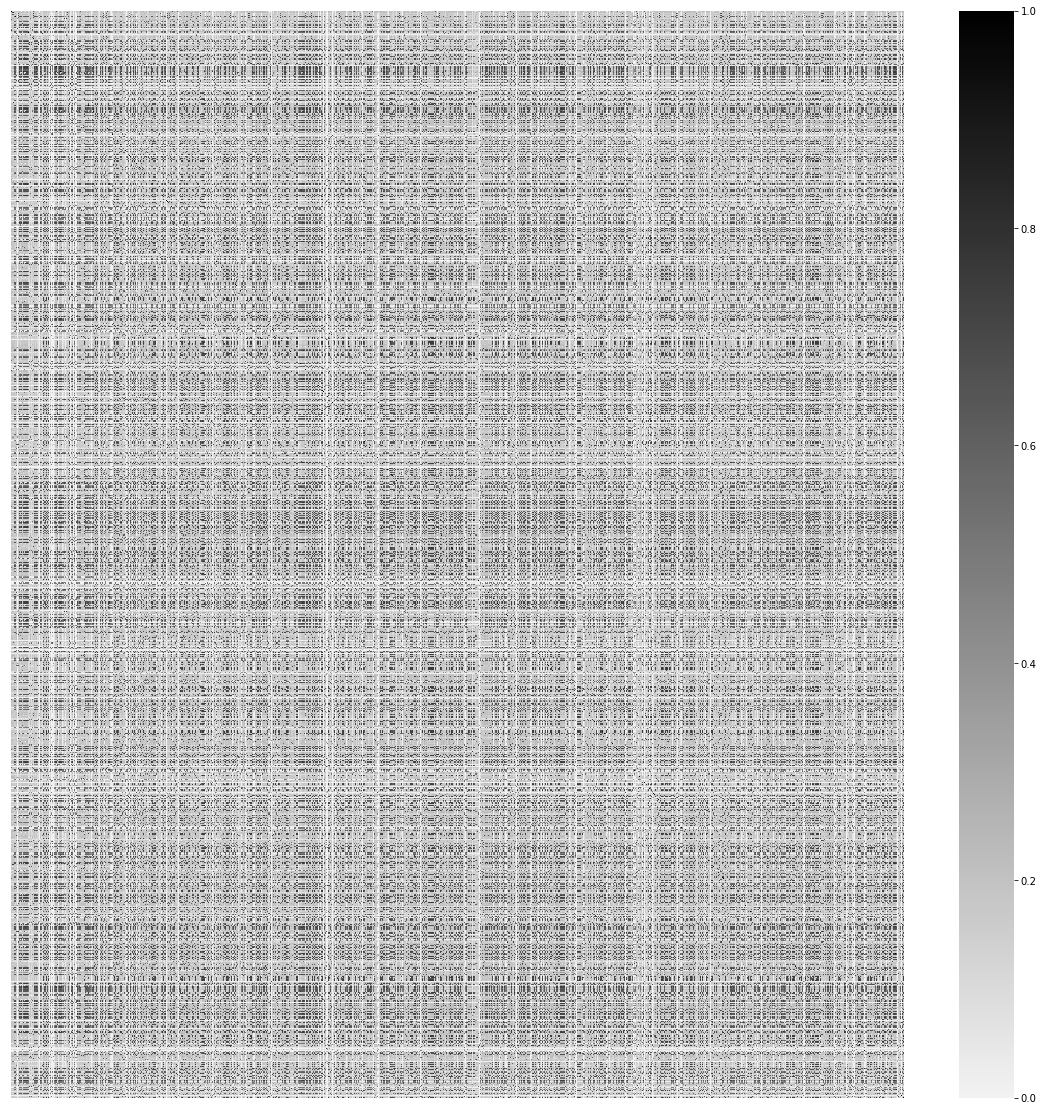
\includegraphics[width=6cm]{event_sim.png}
  \caption*{热力图}
  \label{ff1}
  \end{minipage}
  \begin{minipage}[t]{0.48\textwidth}
  \centering
  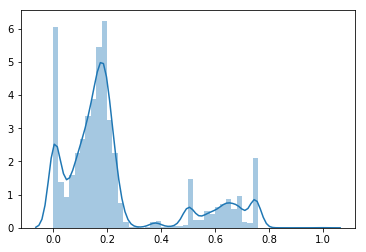
\includegraphics[width=6cm]{event_sim_dist.png}
  \caption*{分布}
  \label{ff2}
  \end{minipage}
  \caption{实验结果}
\end{figure}

可以看出相似矩阵值在0.5附近有较大的差异,并且分布比例也恰好在8:2左右,因此我们把阈值取为0.5。然后我们通过事件成功的定义来对所有事件的成功性进行标注。

\subsubsection{训练分类器}
为了初步的衡量事件的描述对事件参与人数的影响,我们可以将描述作为一个可选的属性,使用一些常用的分类器,例如随机森林,adaboast,对事件成功性进行预测。这里输入是向量化后事件的属性,输出是之前的标注结果。为了避免稀疏高维的文本向量对分类效果的影响,这里对文本的处理方式参考了第二节所用的方法,即事先训练好一个拉索回归器,使用该回归器产生的值来取代原始文本。关于分类器的介绍可以参考附录A。

最终我们使用adaboost,决策树,knn和随机森林作为分类器,使用4折交叉验证来衡量结果,使用网格搜索来确定最佳参数。
本次实验平台为i5-4200m,内存为8G,显卡为gtx-730m。实验结果如图(\ref{f3}):

\begin{figure}
\centering
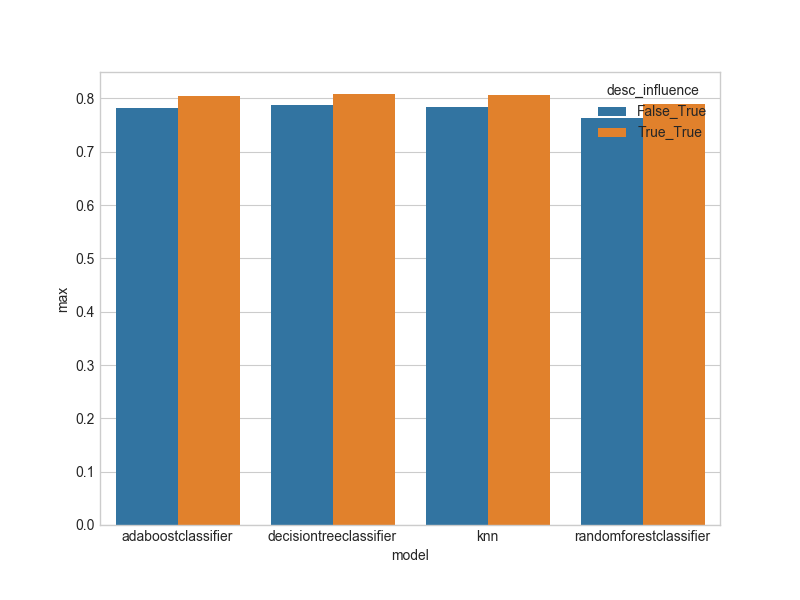
\includegraphics[width=10cm]{exp4_with_1.png}
\caption{}
\label{f3}
\end{figure}

通过实验结果可以看出,加入了事件描述后,分类的精度有了提高。注意到这里排除了相同事件,所以提高的原因不是因为相同事件之间参与人数的相似性。由此可以得出结论:事件描述对预测事件成功起正面作用。

但同时我们也可以看出,事件描述对结果的提高是有限的。这是由于多种原因造成的:一是由于文本处理的方式过于粗糙,二是由于样本太少(交叉验证时每次训练量大概只有3000条),三是由于样本分布不均匀(大概75\%的事件是负样本)。除此以外还有一个很重要的原因:事件描述在某些情况下并不是那么重要。能影响事件参与人数的因素非常多,而在某些情况下,当其他因素起决定性作用的时候,事件描述的好坏就不再是那么重要的了。

想要说明事件描述的影响,光凭分类结果的提升是不够的,引入事件描述对结果最直接的影响是引入了更多的信息,从而提高了分类结果,但有可能并没有提高模型的解释度。为了解决这个问题,我们又设计了如下实验。在介绍接下来的实验前,我们先简单介绍一下线性混合模型。

\subsubsection{线性混合模型}

线性混合模型(\textit{Linear mixed model})是对线性模型的扩展。通过增加固定效应和随机效应,线性混合模型能很好的表示数据中某些非独立的属性对结果的影响。例如性别对于身高来说就是非独立的属性。而对应本文中所使用的数据,就是事件种类,举办地点等属性作为离散变量对于事件参与人数是非独立的。但是事件描述和组内人数则是相对独立的,因此在这里使用线性混合模型来描述这些属性和参与人数的关系是非常自然的一件事情。

\subsubsection{建立混合模型}

为了能更进一步的说明事件描述的加入提高了模型的解释能力,我们使用了混合模型对参与人数与事件的属性之间的关系进行描述。注意到这里我们并不是想根据事件去推算参与人数,而是想给予此判断事件描述在整个模型中起的作用。我们建立的混合模型如下:

\begin{equation}
y_{ijkm}=\beta_0+log|g_i^m|+\gamma_j+\alpha_k+ (\phi_m) +\epsilon_{ijkm}
\end{equation}

其中\(\gamma_j\),\(\alpha_k\)和\(\phi_m\)为事件主题,事件举办人和事件描述的随机效应,固定效应为组内人数。这里没有将事件举办地点纳入考虑范围是因为事件举办地点太多,大多数情况下事件的举办地点都不一样,如果将其考虑进来,会使样本过于稀疏,降低模型的解释性。

Nakagawa和Schielzeth\cite{nakagawa_ageneralandsimplemethodforobtaining_2013}提出了衡量混合模型中的确定系数\(R^2\),在混合模型中,确定系数分为两种,一是\(R_m^2\),衡量固定效应对模型的作用,二是\(R_c^2\),衡量所有效应对模型的作用。计算方法如下:

\begin{equation}
R_m^2=\frac{\sigma_m^2}{\sigma_m^2+\sigma_\gamma^2+\sigma_\alpha^2+(\sigma_\phi^2)+\alpha_\epsilon^2}
\end{equation}
\begin{equation}
R_c^2=\frac{\sigma_m^2+\sigma_\gamma^2+\sigma_\alpha^2+(\sigma_\phi^2)}{\sigma_m^2+\sigma_\gamma^2+\sigma_\alpha^2+(\sigma_\phi^2)+\alpha_\epsilon^2}
\end{equation}

其中\(\sigma\)为方差。我们使用了R语言中的``lme4''计算包\cite{lme4}实现模型,\(R^2\)的计算使用了R语言中的``MuMIn''计算包\cite{MuMIn}。结果如表(\ref{t3})。

\begin{table}[htbp]
	\centering
  \caption{}
  \label{t3}
	\begin{center}
    \begin{tabular*}{\linewidth}{p{0.33\linewidth}p{0.33\linewidth}p{0.33\linewidth}}
  \toprule
                           &  \(R_c^2\) & \(R_m^2\) \\ 
  \midrule
		包含事件描述                       & \textbf{0.653} & 0.135 \\ 
    不包事件含描述                        & 0.494 & 0.135 \\ 
  \bottomrule
    \end{tabular*}
  \end{center}
\end{table}

可以看出包含事件描述后,\(R_c^2\)显著提高,这说明加入了事件描述后,模型的解释性得到了增强。另一个值得注意的是组的规模对事件参与人数并没有特别显著的影响。

\subsection{小结}
本文定义了事件相似性,并使用拉索回归对事件描述进行回归,得到了可解释的结果。然后使用一系列分类器证明了事件描述可以帮助提高预测事件参与度的准确率,最后使用了混合模型证明了该提升并不只是增加了多余的信息,而是提高了模型的解释能力,由此得出事件描述是影响事件是否成功的非常重要的一环的结论。因此,正如前文所描述的,写好一个事件描述,对于sh

然而,值得注意的是,这里我们使用的方法仍然是十分简略的,拉索回归虽然可以得到可解释性的结果,但其简单的特性也导致了其会损失很多信息,例如文本中的序列信息。而这些信息对于提升事件参与度的判定是十分重要的。所以接下来,我们会去尝试更复杂的模型,看看能否在不考虑其他因素的情况下,仅凭借事件描述这一属性,就推测出事件的参与度来。这在现实中也是有意义的:事件组织者可以借助这种工具来预估事件参与人数,以更好的准备举办事件的前期工作。这部分工作将在第二章得到足够多的阐述。

另一个值得注意的地方是如何产生更好的事件描述的工作。近年来在机器翻译,新闻自动撰写等方面的文本生成工作获得了长足的发展,借助序列到序列和对抗网络,我们可以生成可用的,质量足够高的文本。这也启示了我们:一方面,帮助事件组织者判断他们的事件描述是否足够好是有意义的工作,但是如果能自动生成一些有意义的事件描述,也是件有趣的事情。我们将在第三章介绍这部分工作。

总的来说,通过上述实验和方法,我们验证了事件描述对事件参与度是有显著影响的。

\end{document}
% \documentclass[12pt]{template}
% \begin{document}
\section{使用事件描述预测事件参与人数}
\subsection{本章概述}
在这一章中,本文将进一步研究事件描述和事件参与度的关系。上一章的实验证明了事件描述对事件参与度有显著的影响,并且能够帮助提高事件结果的预测结果。如果本文能够更近一步,直接通过事件描述来预测事件参与人数,将会是更有意义的工作。

而在上一章中,本文将事件描述看做词的集合,从而使用了拉索回归作为文本处理方式。而如果我们能用更精细的方式去处理文本属性,将文本的序列信息也纳入考量,那么预测事件结果的准确率也理应有所提高。

所以,为了提高预测事件结果的准确率,同时尝试直接通过事件描述来预测事件参与人数,需要使用更精细的算法来处理事件描述。本文对新的算法的首要考量是要能处理序列信息。因为序列信息是文本很重要的一部分。另一个考量是要有足够的泛化性能,不能过拟合。所以在这里本文使用了卷积神经网络和GRU来设计预测算法。

接下来本章会尝试三种预测算法来预测事件描述和事件参与人数之间的关系。这三种预测算法分别是线性回归,带卷积层的神经网络和带GRU的神经网络。在实验中,本文将先考察这三类预测器在实际数据集上预测参与人数的表现,然后,这三个预测器将会被用在上一章的预测事件结果的实验,用来代替之前处理文本的方法,以考察预测成功率是否有所提高。

\subsection{问题描述}
在本章中,本文主要研究如何仅根据事件描述预测事件参与人数。即给定事件$e_i$和其描述$e_i^d$,通过某个函数$g$,来使$\bigtriangleup(g(e_i^d),|e_i^a|)\to 0$。其中$g$即为本文需要设计的预测算法。从这个角度来看,这个问题是个典型的回归问题。
\subsection{线性回归预测器}
线性回归是最简单的一种回归方法,而且只要二者关系是正相关的,在大多数情况下线性回归也有着不错的效果,因此,这里选择线性回归作为预测算法。同时,线性回归也是本次实验的基线(\textit{baseline})。在实验中,本文并没有采用最传统的线性回归,而是采用了拉索回归。原因是为了与上一章的文本处理方式保持一致。所以这里在损失函数中加入$\mathrm{L1}$正则来突出某些词的作用。此预测器及其损失函数如下:
% lasso function
\begin{equation}
argmin\left\{\frac{1}{N}\displaystyle\sum_{i=1}^{N}
(y_i-\beta_0-\displaystyle\sum_{j}\beta_jx_{ij})^2\right\}
\end{equation}
\begin{equation}
subject\ to \quad \displaystyle\sum_{i}|\beta_i|<\alpha
\end{equation}
\begin{equation}
loss\ function: \mathrm{MSE}+\sigma*\sum|\beta|
\end{equation}

在实现中,为了与后面两个分类器统一,本文使用了输出维数为1的单层线性神经网络,并采用了L1正则。预测器的输入是序列化后的文本,目标(\textit{target})及输出则是参与人数。


\subsection{带卷积层的神经网络}
\subsubsection{卷积层在自然语言处理中的运用}
卷积神经网络通常被用在图像处理中,但它在自然语言中也有很多运用。在图像处理中,卷积层的输入通常是像素,然而在自然语言处理中,它的输入在更多情况下则是由句子组成的二维矩阵。矩阵的行通常是词语,矩阵的列则是该词所对应的向量。本文使用独热编码来表示每一个词,但更多的情况下则是使用词向量。例如如果一句句子中有20个词,而词向量的维度为200,则卷积层的输入就是一个$20*200$的矩阵。

在设置卷积核的大小时,本文将卷积核的宽度设置成词向量的维度,而将卷积核的高度设置在2\~5左右。所以在进行卷积操作时,与图像处理的卷积层不同,自然语言处理中的卷积通常只会向一个方向滑动。

卷积层之所以有效,是因为它能处理局部相关的信息。而自然语言也部分符合这一要求:靠得近的两个词很有可能存在着某种语义上的关联。虽然在自然语言中可能存在例外情况,比如语义上有联系的文本被几个无意义的词隔开。但这并不妨碍卷积层在自然语言处理中的广泛应用。比如文本分类,垃圾邮件检查,主题分类等。
\subsubsection{网络结构}
在使用线性回归做预测器时,本文假设文本序列中各属性对结果的影响是互相独立,不受出现顺序影响的,即\(d(w|s_0)=d(w|s_0')=d(w)\),其中\textit{w}为词,\(s_0,s_0'\)为不同排列的相同的文本序列,\textit{d}为某个影响函数。但显然这个假设在现实中是不成立的,在自然语言中,词的出现顺序是非常重要的信息。例如在一段事件描述中,\textit{we will hold the meeting in a church}与\textit{church a in meeting the hold will we}这两句话在上一节的线性规划预测器的眼中是没有区别的,但以自然语言的角度看,第二句话是没有意义的。因此,为了将文本的序列信息纳入考量范围,这里本文参考了seqGan\cite{yu_seqgan:_2016}中判别器的结构,设计了带卷积层的神经网络。
如图\ref{f21}。判别器的具体处理过程如下。

这里本文首先将输入文本\(w_0,w_1,...,w_t\)表示成如下形式:
\begin{equation}
S_{1:t}=x_1\oplus x_1\oplus...\oplus x_t
\end{equation}

其中,\(x_i\)为\(w_i\)对应的\textit{k}维词向量\(\subseteq R^k\),\(\oplus\)是拼接符号,\(S_{1:t}\)是一个\(t\times k\)的矩阵。然后使用若干个卷积核\(k\subseteq R^{l\times k}\)对窗口大小为\textit{l}中的词进行卷积操作,产生一个新的特征向量。
\begin{equation}
c_i=\rho(w\otimes S_{i:i+l-1}+b)
\end{equation}

\(\otimes\)为按元素乘积(element-wise product)之和,\textit{b}为偏移量,\(\rho\)为非线性函数。在实现中本文使用多个相同尺寸的核来进行卷积,然后对得到的不同的\(c_i\)取其中最大的一个,例如图\ref{f21}中第一个卷积核的\textit{l}为3,使用了4个不同的卷积核,即对于相同的窗口一次输出四个结果,然后在这四个结果中取最大值,即为窗口大小为\textit{l}所对应的最终卷积结果。为了得到不同窗口尺寸下的上下文关系,本文使用不同尺寸的核。最后,将结果拼接起来,得到处理后的特征向量。送入下一个环节。下一个环节为带隐含层的线性网络,假设得到最终的特征向量为\(\hbar\subseteq R^{k'}\)(图中对应的\textit{k}为9),那么接下来本文对\(\hbar\)进行如下操作。
\begin{equation}
\hbar'=\sigma(w_0\cdot\hbar+b_0)
\end{equation}
\begin{equation}
output = w_1\cdot\hbar'+b_1
\end{equation}

其中\(w_0,w_1\)分别对应第一和第二个蓝色方块,\(\sigma\)为非线性函数,\(\cdot\)为矩阵乘法运算,\(b_0,b_1\)为偏移量。

关于该网络的损失函数,为了最小化预测结果和目标的误差,本文使用了均方误差损失函数($\mathrm{MSE}$),并对最后两个线性神经网络采用了L2正则(公式(\ref{eq1}))。这里采用L2正则的原因是本文希望最后的线性神经网络能尽可能的考虑前面卷积神经网络输出的所有维度,而不是过度的依赖某些维度来做出判断。
\begin{equation}\label{eq1}
loss=\frac{1}{N}\displaystyle\sum_{i=1}^{N}\left\{(y_i-y'_i)^2\right\}+\alpha||w_0^2||+\beta||w_1^2||
\end{equation}
\begin{figure}[htbp]
    \centering
    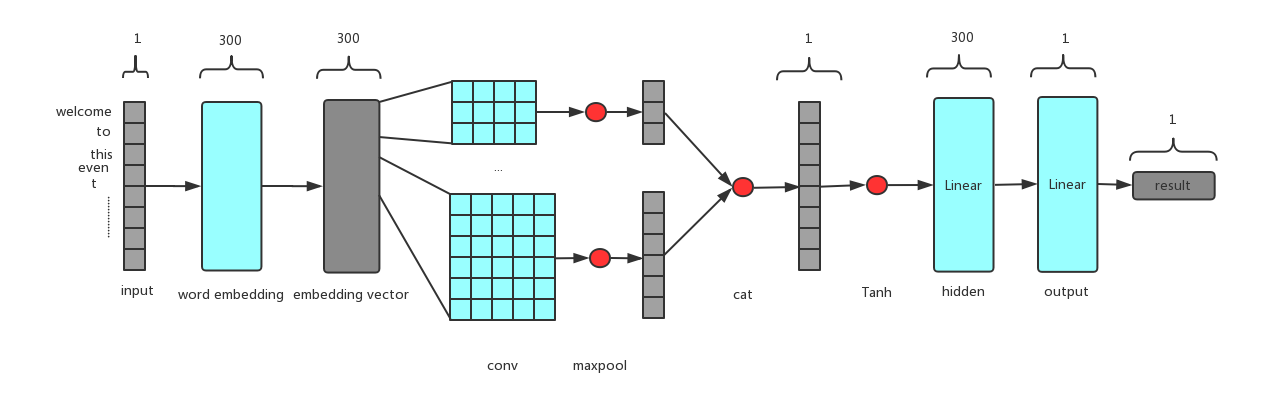
\includegraphics[width=16cm]{conv_ranker.png}
    \caption{带卷积层的神经网络}
    \captionsetup{font=footnotesize,margin=30pt}\caption*{图中灰色的方块表示向量,蓝色的表示网络,红色的圆点表示算符。在计算过程中,输入是文本序列,然后首先经过词向量层转换成词向量,然后进行卷积和池化(max-pooling),将结果拼接起来,然后使用双曲正切(tanh)归一话,最后经过一个带隐含层的线性前馈神经网络输出最终结果。}
    \label{f21}
\end{figure} 

\subsection{带GRU的神经网络}
\subsubsection{RNN在自然语言处理中的应用}
RNN在自然语言处理中运用的十分广泛,是因为它克服了卷积层的弊病。卷积层中由于卷积核感受野的限制,在某些情况下不能很好的收集原始文本中的信息。同时由于自然语言的局部相关性有时候不是那么明显,使用卷积层也不能总是达到很好的效果。而RNN则不同,RNN的感受野是整个句子,同时RNN对文本从左到右(或双向阅读)的处理方式也和人阅读文本时十分类似,所以RNN天然适合自然语言处理。

在实际运用中,为了防止文本序列过长而导致的梯度消失的问题,我们通常会使用RNN的变体:LSTM或者GRU。
\subsubsection{网络结构}
在上一小节,本文使用了卷积层对原始输入文本转换成的词向量进行了处理,得到了一个新的特征向量。这个过程也可以看成是定义了一个函数\(f:R^{m\times k}\mapsto R^n\),将原本在\(R^{m\times k}\)空间中的样本编码到了\(R^n\)中。这样做的目的是可以方便后续处理,相当于把一条文本转换成了一个向量,接下来的工作就在这向量上展开了。但如何去找到一个这样的函数\textit{f},则是这种方法成败的关键。本文希望\textit{f}有如下的特点:1)能处理序列信息。2)能在转换过程中尽量保留原始信息。3)易于实现。而本文之前使用的卷积层并不完全满足这三个条件。首先,它能处理序列信息,但它处理序列信息的能力来源于窗口大小的设置,因此,合理的设置窗口大小非常重要。而在文本处理中,如何设置窗口大小是件困难的事情。其次,因为池化层的存在,它在转换过程中能保留多少原始信息是存疑的。

而另一种处理时序信息的网络结构循环神经网络,则可以很好的满足上面三个条件。所以近年来这种网络也在自然语言处理上得到了广泛的应用,例如在序列到序列模型中,循环神经网络就常常被用在编码/解码环节。同样在这里,本文使用循环神经网络的一种形式$\mathrm{GRU}$\cite{DBLP:journals/corr/ChungGCB14}作为编码器。

\paragraph{GRU}
GRU(gated recurrent network,图\ref{f22})是为了克服传统的循环神经网络中无法很好的处理远距离依赖而提出的$\mathrm{LSTM}$的一个变体。它相较于$\mathrm{LSTM}$来说更加简单,但仍保持着不错的效果\cite{DBLP:journals/corr/ChungGCB14}。GRU的前向传播如公式(\ref{3-9}),公式(\ref{3-10}),公式(\ref{3-11})。其中,\textit{W,U,b}都是参数。\(x_t\)为输入向量,\(h_t\)为输出向量,\(z_t,r_t\)为更新门和重置门向量。同样的,根据链式法则,可以得到其反向传播公式。

\begin{figure}[htb]
    \centering
    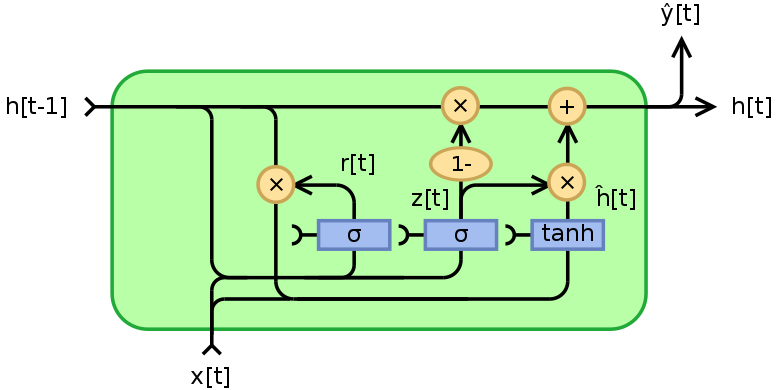
\includegraphics[width=11.5cm]{GRU.png}
    \caption{GRU}
    \captionsetup{font=footnotesize,margin=30pt}\caption*{图中\(z[t]\)为更新门,\(r[t]\)为重置门。\(h[t]\)为当前\textit{t}时刻的隐含状态,橙色的圆点为算符,蓝色方框为某非线性函数}
    \label{f22}
\end{figure}

\begin{equation}\label{3-9}
z_t=\sigma_z(W_zx_t+U_zh_{t-1}+b_z) 
\end{equation}
\begin{equation}\label{3-10}
r_t=\sigma_r(W_rx_t+U_rh_{t-1}+b_r) 
\end{equation}
\begin{equation}\label{3-11}
h_t=(1-z_t)\cdot h_{t-1}+z_t\cdot tanh(W_hx_t+U_h(r_t\cdot h_{t-1})+b_h)
\end{equation}

\paragraph{带GRU的预测器}
将之前的神经网络的卷积层替换成本小节介绍的GRU,本文便得到了另一个新的预测器(如图\ref{f23})。可以看出,该预测器的结构与之前的神经网络十分相似,仅在编码环节有所不同。

\begin{figure}[htb]
    \centering
    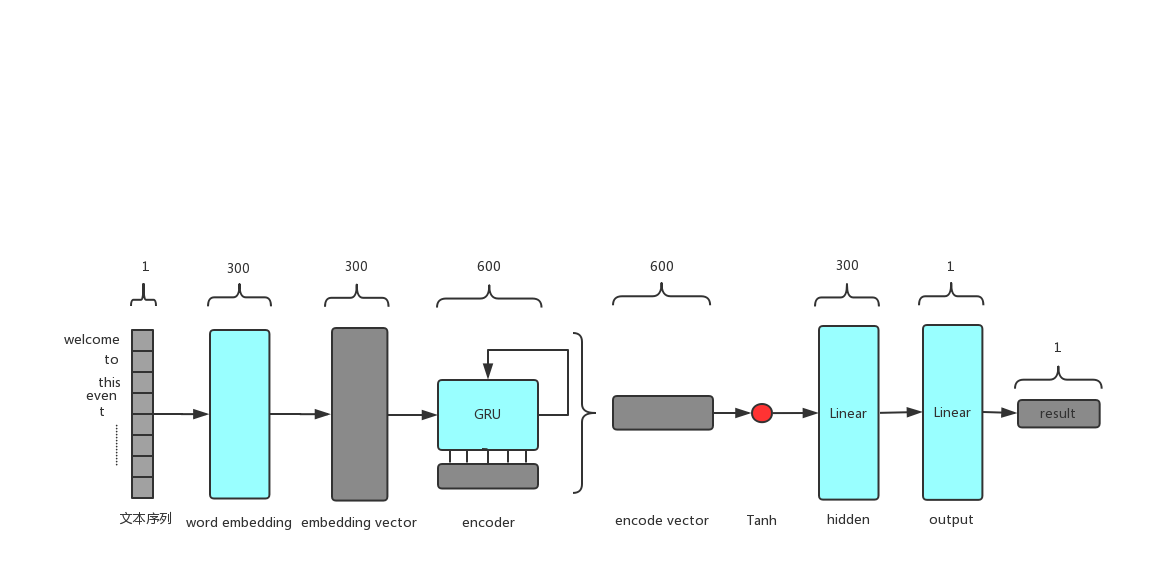
\includegraphics[width=16cm]{gru_ranker.png}
    \caption{带GRU的神经网络}
    \captionsetup{font=footnotesize,margin=30pt}\caption*{图中各色块和圆点的意义同图\ref{f21}。在计算过程中,本文首先将序列转换成词向量,然后使用GRU进行编码,获得一个新的向量(\textit{encode vector}),然后使用双曲正切(\textit{tanh})归一化,最后经过一个带隐含层的线性前馈神经网络输出最终结果。}
    \label{f23}
\end{figure}
\subsection{词向量的初始化}
在自然语言处理中,如何表示词是值得研究的问题。而词向量是指自然语言处理中将词映射到向量的一种方式。在上一章中,本文使用独热编码作为词向量。这种表示方式固然有其简单易实现的特点,但也有维度高,稀疏,词之间相关性差的缺点。因此在本章中,本文使用word2vec\cite{word2vec}算法来计算词向量。

在具体实现中,本文尝试了两种方式来初始化词向量:1)使用gensim中提供的word2vec函数来计算词向量。并使用它来进行初始化。2)使用归一化的服从正态分布的随机数来初始化词向量。实验证明这两种方式并没有显著区别,因此,在实验中,本文采用了第一个方法。
\subsection{实验设计与结果}
在本节中,本文将通过两个实验来比较不同的文本处理方式的效果。在第一个实验中,本文将比较不同的预测器在预测参与人数上的差异:本文首先使用百分之八十的事件训练预测器,并使用剩下的数据对预测器进行评估。在第二个实验中,本文将使用本章提出的预测算法来取代上一章预测事件结果中使用的事件描述评价器,来比较不同的文本处理方式对预测事件结果准确率的提升。
\subsubsection{数据集,评估方式及参数设置}
本次实验所使用的数据集与上一章完全相同。本文所用的数据集来自meetup的LA市,包含超过20万个事件,数据集的详细情况见表\ref{t1-1}。在评估方式上,针对第一个实验,本文使用了均方误差来衡量预测值和参与人数的距离。在第二个实验中,和上一章相同,本文仍使用准确率作为评价指标。在参数设置方面,本文使用了网格搜索和四折交叉验证的方式,确定了最佳参数如表\ref{t2-1}所示。

\begin{table}[htb]
\caption{\label{t2-1}网络参数设置}
\centering
\begin{tabular*}{\linewidth}{p{0.333\linewidth}p{0.333\linewidth}p{0.333\linewidth}}
\toprule
    参数         & 带GRU的神经网络 & 带卷积层的神经网络 \\
\midrule
    词向量维度      & 300       & 300       \\
    GRU的\(h_t\)维度   & 600       & 无         \\
    卷积核窗口大小    & 无         & 1,2,3,4,5 \\
    线性神经网络隐层维度 & 300       & 300      \\ 
\bottomrule
\end{tabular*}
\end{table}

\subsubsection{实验结果与分析}
\paragraph{实验一的结果与分析}
本文使用了百分之八十的事件训练预测器,并使用剩下的数据对预测器进行评估。训练及测试过程的损失函数变化如图\ref{f2-4}。
\begin{figure}[htb]
	\centering
	\begin{subfigure}{.49\textwidth}
		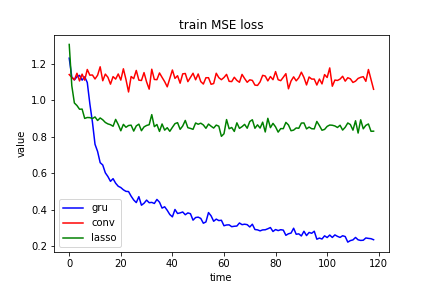
\includegraphics[width=\textwidth]{trainloss.png}
		\caption{train MSE loss}
	\end{subfigure}
%%%%%%%%%%%%%%
	\begin{subfigure}{.49\textwidth}
		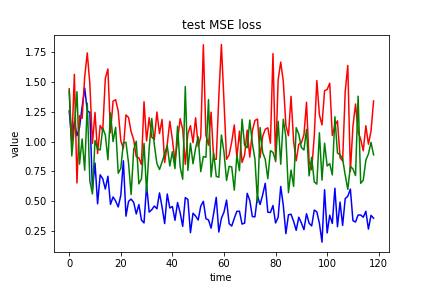
\includegraphics[width=\textwidth]{testloss.png}
		\caption{test MSE loss}
	\end{subfigure}
    \caption{实验结果,其中纵轴为参与人数(对数),横轴为循环次数(×100)}
    \label{f2-4}
\end{figure} 
从图中可以看出,使用GRU作为编码器的神经网络的表现最好,其次是线性预测器,使用卷积层的神经网络表现最糟糕。这点是出乎意料的,原因可能是卷积层在自然语言处理中比较适合短文本分类,即能区分文法上有明显区别的句子。但由于其感受野的限制,不适合用来区分整个文本的语义区别。而另一点值得注意的是尽管GRU在此次实验中的表现最好,但是其结果仍然不是特别理想(从测试环节损失函数的曲线的抖动也可以看出这一点)。这是因为在预测过程中本文仅使用了事件描述这一属性,而没有参考其他属性,例如事件种类,所在组别,举办时间,举办地点,举办者等。属性的缺失限制了这些预测器的上限。如果在预测时加上了这些属性,参考第一章,可以预见准确度应该会有所提升。 
\paragraph{实验二的结果与分析}\label{train_discrimiator}
本次实验的数据集和分类算法与第二章所采用的方式完全一致,仅在处理文本时使用本章提出的使用GRU作为编码器的神经网络。本次实验仍使用百分之七十的数据作为训练数据,剩余的百分之三十则用来评估分类结果。本次实验使用交叉验证和网格搜索的方式来确定最佳参数,实验结果见表\ref{t2-2}。

\begin{table}[htb] 
    \centering
    \caption{\label{t2-2}使用不同文本处理方法和分类器对预测事件结果的影响}
    \begin{tabular*}{\linewidth}{p{0.2\linewidth}p{0.2\linewidth}p{0.25\linewidth}p{0.25\linewidth}}
\toprule 
分类器&不包含事件描述&使用拉索回归处理文本&使用GRU神经网络处理文本\\
\midrule
Adaboost & 0.762 & 0.791 & 0.801 \\
Decision Tree& 0.763 & 0.786 & 0.811\\
Knn & 0.764 & 0.782 & 0.799 \\
Random Forest & 0.762 & 0.788 & \textbf{0.830} \\
\bottomrule
    \end{tabular*}
\end{table}

实验结果可以看出,使用$\mathrm{GRU}$作为编码器的神经网络来处理事件描述的准确率最高,其次是使用拉索回归处理。排除事件描述作为分类属性的结果最差。所以,在使用了新的文本处理方式后,预测事件成功率的准确度有所提高。这反过来也证明了事件描述在事件成功/事件参与人数上的重要作用。
\subsection{本章小结}
本章主要研究了不同的事件描述处理方式对预测事件结果和事件参与度的影响。实验证明,使用GRU的神经网络无论在预测事件参与人数的精度上还是在预测事件结果上都要高于其他两个预测器。这也证明了循环神经网络在处理时序信息上的能力。

与此同时,我们还可以看到,光凭事件描述是无法很准确的预测事件参与人数的。因为哪怕是排除了事件描述,事件其他属性的随机效应的确定系数也达到了0.494。这说明了其他属性在决定事件参与度上也是很重要的,而如果缺失了这一部分信息,自然无法准确的预测出事件参与人数来。

在下一章,本文将提出一个带变分编码器的端到端的网络作为事件描述生成模型,使用本章的带GRU的神经网络作为判别模型。这两个神经网络将被运用在一个生成对抗网络中,以训练出可以生成新的事件描述的网络模型。
% \end{document} 
\documentclass[]{template}
\begin{document}
\section{生成事件描述}
\subsection{本章概述}
在前两章,我们首先验证了事件描述对事件成功的影响,并通过事件属性预测了事件结果,以及衡量了事件描述与事件参与人数的关系。后者对于事件组织者尤为重要,因为一个组织者总是会关心他的活动会有多少人参加。而另一个事件组织者十分感兴趣的话题是他该如何写出好的事件描述。因此,如果能够根据历史数据,来自动生成一些事件描述供组织者参考,是十分有意义的。

本章在上一章的基础上,设计了一个生成模型(\textit{generator}),用来生成事件描述。在考察了诸多文本生成模型后,我们在本文使用了变分自编码器\ref{kingma_auto-encoding_2013,bowman_generating_2015}(\textit{variational autoencoder})。这里使用变分自编码器的原因是因为我们希望文本在编码空间内服从我们期望的分布,具体的来说,我们希望每段文本的隐编码的周围是连续的,同时不同文本的隐编码在隐空间间也是连续的,这样的话可以避免传统编码器所带来的一些问题,比如样本在隐空间的分布不连续,导致只无法在隐空间采样来生成文本。然后我们使用上一章设计的基于GRU的神经网络作为判别器(\textit{discrimitor}),组成一个生成对抗网络\ref{goodfellow_generative_2014}。由于在训练时借鉴了强化学习中的策略梯度下降\textit{policy gradient},因此我们将其命名为GAN\_PG,通过设计合理的奖励函数,来训练生成器生成好的事件描述。

本章的结构如下:首先我们会详细介绍文本生成模型的设计和训练过程,然后我们会对GAN\_PG中使用的生成模型以及其奖励函数进行详述,最后我们会在真实的\textit{meetup}数据集上给出实验结果。

\subsection{事件描述生成模型}
\subsubsection{循环神经网络语言模型}
循环神经网络语言模型(\ref{RNNLM})是目前十分流行的一种语言模型。在生成句子时,RNNLM仅根据当前隐层的状态给出下一个词的概率分布,而不是其他假设。而RNN模型本身又十分强大,几乎可以拟合任何分布。而自然语言在某种程度上又可以看成一个概率模型,每一个词出现的概率都由之前已出现的词决定,因此,只要有训练数据,RNNLM就可以很好的对复杂文本序列建模。反应在实验中就是其生成的文本十分像它的训练数据,例如如果我们使用莎士比亚的文章作为训练数据,那么其生成文本读起来也像莎士比亚。这种性质也让它在文本生成器中得到了广泛应用,几乎所有的序列到序列(\textit{seq2seq})模型中的解码器(\textit{decoder})都采用了RNNLM。本文也不例外。
\subsubsection{变分自编码器}
RNNLM在生成文本序列中的某一个词时,完全依赖于之前输入的词和隐状态。而在实现中,通常会使用一个特殊符号来作为每一句的开头,因此,RNNLM生成的文本序列完全依赖于其刚开始时的隐状态。所以如何提供合适的隐状态来使生成的句子符合预期,就显得尤为重要了。一个解决方案是使用第二章提到的GRU编码器。编码器首先将输入序列编码到一个隐空间,然后使用一个前向神经网络将这条编码转换成RNNLM初始化的隐状态。但是这样做有一个非常明显的缺陷:我们无法控制输入样本经过编码器编码后在隐空间中的分布。在原空间相似的两个文本序列在编码后它们所对应的隐向量可能并不相近。这显然不是我们期望的。另一方面是,GRU在编码过程中,是直接算出对应文本序列的隐编码,而非采样获得,这就导致了隐编码在隐空间中是不连续的,换而言之,在隐空间中可能只有几个点有意义。因此,在这里仅依靠GRU编码器是不够的。但是我们可以使用变分编码器,它是传统的RNN编码器的改进型,它对隐空间中的编码\(\overrightarrow{z}\)加入了先验分布,并在目标函数中通过kl散度来缩小实际分布和先验分布的距离,以此来强迫编码器学到合适的编码方式。同时,它通过采样来生成编码,这也就保证了隐编码周围的点也都是有意义的。变分自编码器的损失函数$L_i(\theta,\phi)$如\ref{3-1}
\begin{equation}\label{3-1}
    L_i(\theta,\phi)=-E_{z\sim q_\theta(z|x_i)}[\log p_\phi(x_i|z)]+KL (q_\theta(z|x_i)||p(z))
\end{equation}
可以看出,其损失函数由两部分构成,第一部分是负对数似然损失函数,用来缩小输入序列和输出序列的差异。第二个部分则是kl散度,其中$q_\theta$为编码器,$p(z)$为对隐编码$z$的先验分布。

\subsubsection{事件描述生成模型}
我们参考了\ref{bowman_generating_2015},设计了如下事件描述生成器(这里缺张图)\ref{}。在编码器和解码器的选择上,我们都使用了单层GRU。在实现过程中,我们使用$0-1$高斯分布作为隐编码的先验分布。同时使用了重采样\ref{kingma_auto-encoding_2013}的技巧,这样我们便可以用反向传播来训练我们的网络:在抽样的时候,我们不直接对隐编码进行采样,而是通过两个线性神经网络获得当前编码的平均值$\bar{u}$标准差$\bar{v}$,然后通过公式\ref{3-2}获得隐编码,其中$\bar\epsilon \sim Normal(0,1)$。
\begin{equation}\label{3-2}
    z=\bar{u}+\bar{v}\odot \bar\epsilon
\end{equation}

至于如何使用前半段编码结果来初始化解码器中的隐状态,我们尝试了三种方法1)将隐编码连接在解码器的输入词向量的最后。2)将隐编码通过一个前向网络转换成解码器的隐状态向量,并用它直接初始化后者。3)两者皆做。在实际运用过程中,我们发现这三种方法并没有很大的差别,因此最终我们采用了第一种方案。

在实际的训练过程中,为了防止损失函数中KL散度降为0,我们还参考了\ref{bowman_generating_2015}中所采用的策略:在训练刚开始时设置KL散度项的权重为零,然后慢慢升到一。这样训练过程其实就分成了两个阶段:第一个阶段,编码器从文本序列中学到尽可能多的信息,但不保证分布符合先验分布。第二阶段,通过增加KL散度项的权重,强迫编码器编得的隐编码尽可能接近先验分布。

\subsection{GAN\_PG}
通过前文的事件描述生成器,我们可以生成读上去通顺的事件描述。只要训练数据是文法通顺的句子,那么输出也会是文法通顺的句子。我们有两种方式可以获得事件描述:一种是在隐编码空间里面随机采样。这样生成的事件描述文法通顺,但无法保证语义上的一致。另一种是在已知事件描述的隐编码周围采样,由于采用了变分自编码器,相似的文本序列的隐编码在隐空间中也是相近的。因此,如果我们采用第二种方法,仅在已知事件描述隐编码的周围采样,我们便可以获得和已知事件描述在文法上一致的新的事件描述。如果我们能找到一种方法,使每次的改变都往我们期望的方向上发生,便可以起到改进事件描述的作用,正如\ref{noauthor_sequence_nodate}中做的一样。而借助上一章的预测器,我们可以预测新的事件描述的参与人数。而通过设计合理的奖励函数,我们可以让解码器学到如何生成能够在预测器上获得高分的文本序列。但这样做有一个问题:我们不能保证预测器是可靠的,即在预测器上获得高分的文本序列可能并不符合我们的期望,因此在训练生成器的同时,我们还要对预测器进行训练,使之能正确的区分真正的样本和生成的样本,这便是此处用到生成对抗网络的原因了。
\subsubsection{生成对抗网络简介}
生成对抗网络(\textit{Generative Adversarial Net}\ref{goodfellow_generative_2014})是Goodfellow于2014年提出的。它包含生成(\textit{generator})模型和判别(\textit{discrimitor})模型。在训练过程中,生成模型的目标是生成能够让判别模型无法分辨出其和真实数据的区别样本,而判别模型的训练目标则是将生成模型生成的假样本从真实样本中区分开来。在标准的生成对抗网络中,我们最大化判别模型正确分类的概率,同时最小化生成模型所生成的样本被判别器正确分类的概率,目标函数见\ref{3-3}。
\begin{equation}\label{3-3}
    \mathop{min}_G \mathop{max}_D V(D,G)=E_{x\sim data}[\log D(x)]+E_{x'\sim G_\theta}[\log(1-D(x')]
\end{equation}

其中,$D,G$分别表示判别和生成模型,$data$表示真实数据集。$G_\theta$表示生成模型产生的假数据。
\subsubsection{GAN\_PG}
GAN\_PG的生成模型为本章第二节介绍的事件描述生成模型,判别模型为上一章介绍的带GRU的神经网络。判别模型的损失函数为最小化\ref{3-4}式(即在\ref{3-3}前加上负号)。
\begin{equation}\label{3-4}
    \mathop{min}_D-E_{x\sim data}[\log D(x)]-E_{x'\sim G_\theta}[\log(1-D(x')]
\end{equation}
生成模型的损失函数为最大化\ref{3-5}式。其中$G_\theta,D_\sigma$分别为生成模型和判别模型,\ref{3-5}式的前半部分为在隐编码$z$和已生成的序列$y_{0:t-1}$下,生成当前$y_t$的概率。\ref{3-5}式的后半部分为生成模型生成$y_t$在判别模型所获得的评分。最大化\ref{3-5}式即最大化生成模型在生成序列的每一步中所获得的评分。
\begin{equation}\label{3-5}
pg\_loss=\mathop{min}\sum_{\substack{t}}-\log G_\theta (y_t|z,y_{0:t-1})*D_\sigma (y_t,y_{0:t-1})
\end{equation}

接下来的问题是如何衡量生成模型所生成的每一步获得的评分。因为判别模型只有在生成模型生成完整个序列以后,才能对该序列评分,而\ref{3-5}式所要求的是实时的评分。在本文中,参考\ref{yu_seqgan:_2016}中所用的方法,我们使用了策略梯度来设计损失函数:对于$t$时刻所生成的序列$y_t$,我们使用了策略网络$G_\theta$(即当前生成模型)通过蒙特卡洛搜索算法对接下来$T-t$项(T为序列长度)进行采样,即式\ref{3-6}。
\begin{equation}\label{3-6}
    \{y_0,y_1,\dotsb,y_T\}=\mathrm{MC}^{G_\theta}(y_{0:T})
\end{equation}

其中$y_{0:t}$为当前状态,$y_{t+1:T}$为基于当前生成器装态采样的结果。为了获得更准确的结果,我们可以将上述过程重复数次,取平均。经过改进的生成模型目标函数如式\ref{3-7}。
\begin{equation}\label{3-7}
D_\sigma(y_t,y_{0:T-1})\sim 
\begin{cases}
    D_\theta(y_{0:T-1}) & \text{if } t =T-1 \\
    \mathrm{E}(D_\theta(y_{0:t-1}:y_t:y_{t+1:T-1})),y_{t+1:T-1}\sim \mathrm{MC}^{G_\theta}(y_{0:t}) & \text{if }t<T-1
\end{cases}
\end{equation}

在确定了判别器,生成器和其分别的目标函数后,我们通过算法\ref{s3-1}来训练GAN\_PG。
\linespread{0}
\begin{table}[htbp]
    \label{s3-1}
    \begin{center}
        \begin{tabular*}{.75\linewidth}{p{0.75\linewidth}}
\toprule
            算法一、训练GAN\_PG \\
\midrule
\begin{minipage}[t]{\linewidth}
\begin{enumerate}[itemsep=-2pt]
    \item 预训练生成模型
    \item 预训练判别模型
    \item \textbf{repeat}
    \item \quad \textbf{for} g-step \textbf{do}
    \item \quad \quad 使用$G_\theta$生成序列$S_{0:T}$
    \item \quad \quad 使用式\ref{3-5}计算目标函数
    \item \quad \quad 更新参数$\theta$
    \item \quad \textbf{end for}
    \item \quad \textbf{for} d-step \textbf{do}
    \item \quad \quad 采集\textbf{n}个负样本,\textbf{m}个正样本
    \item \quad \quad 计算与目标的均方误差
    \item \quad \quad 更新参数
    \item \quad \textbf{end for}  
    \item \textbf{end for}
\end{enumerate}
\end{minipage}\\
\bottomrule
        \end{tabular*}
    \end{center}
\end{table}
\linespread{1.3}

\subsection{实验}
在本小节,我们将在真实的数据集上验证我们的方法,本章采用的数据集和第一,第二章相同,在此不多做介绍。本章的结构将分为两个部分,第一部分阐述事件描述生成模型,即生成模型的预训练,第二部分描述判别模型和GAN\_PG的训练。
\subsubsection{训练事件描述生成模型}\label{train_generator}
\paragraph{训练细节}
在训练事件描述生成器时,我们要保证其目标函数(\ref{3-1}的两部分处在合适的平衡状态。因为一方面我们前半项越小越好,另一方面我们又希望后半项较小又不太小。保证前半项足够小是为了缩小和训练样本的距离,后半项相对较小是为了让其隐编码服从特定分布,但如果后半项太小,则不同训练样本的隐编码过于相似(都接近0-1高斯分布),也失去了编码器的意义。所以我们使用文提及的方法,在训练过程中让后半项的权重为0,先训练前半项,再慢慢将后半项的权重增加,以训练后半项。在实现过程中,我们用了式(\ref{3-8})来调整后半项的权重,同时为了使后半项值能稳定在合适的范围,我们将前半项的系数设置为79。训练的前半项,后半项以及$\mathrm{KL\_Weight}$的变化图如图\ref{}(这里少张图)。接下来,我们将对训练好的生成器进行实验。我们将做两个实验:对已知样本的采样和随机采样。
\begin{equation}\label{3-8}
    \mathrm{KL\_Weight}=\frac{\tanh\frac{i-3000}{1000}+1}{2}
\end{equation}

\paragraph{对已知样本采样}  
在本节中,我们将对已知样本的隐编码$z \sim \mathrm{p}(z|x)$进行采样,其中$x$为已知的文本序列,即事件描述。$\mathrm{p}(z|x)$为编码过程。我们通过式(\ref{3-2})进行采样。通过此举,我们可以对生成器认为的相似的句子有个大概的了解。实验结果如表\ref{t3-2}所示。 
\begin{table}[htbp]
    \center
    \caption{\label{t3-2}对已知样本采样的结果}
    \begin{tabular*}{\linewidth}{p{0.2\linewidth}p{0.8\linewidth}}
\toprule
样本一 & we are meeting at the actual merry go round <ukn> . \\
对隐编码解码 & we will be meeting at the corner of the park entrance .\\ 
采样一 & we will be meeting in the back room , and then the <ukn> will be on the right hand side of the stage .\\
采样二 & we are going to have a great time of year 's theme for the day . \\
采样三 & we will be meeting at the end of the day before the show . \\
\midrule
样本二 & we 'll be there the whole night . \\
对隐编码解码 & we will have a dj spinning the best of the night !\\ 
采样一 & we 're going to have a great turnout .\\
采样二 & the presentation will be on the right side of the road .\\
采样三 & after the concert we 'll have a chance to visit the bars in the park . \\
\bottomrule
    \end{tabular*}
\end{table}
\paragraph{随机采样}
本节中,我们将对未知的隐编码进行采样,同时检验在编码空间中相邻点的编码结果的语义一致性和文法一致性。我们先在隐空间中进行采样,获得隐编码$z_1,z_2 \sim \mathrm{Normal}(0,1)$,然后我们在两点间进行线性插值,获得编码集合$\{z_i\} = t*z_1+(1-t)*z_2 ,\mathrm{for}\ t \in [0,1]$。随后我们再对集合$\{z_i\}$进行采样,采样结果见表\ref{t3-3}。借助此举,我们可以了解到在隐空间中,相临隐编码在解码后的文本序列上的相似性和主题的一致性。 

\begin{table}[htbp]
    \center
    \caption{\label{t3-3}随机采样结果(加粗部分为起点和终点)}
    \begin{tabular*}{\linewidth}{p{\linewidth}}
\toprule
\textbf{the event is free , but donations will be greatly appreciated .}\\
the event is free , but you must rsvp on meetup . \\
we 'll be meeting at the corner of the santa monica pier and walk to the parking lot .\\
join us for a fun evening of the evening !\\
\textbf{join us for a fun evening of dancing , fun , and fun !}\\
\midrule
\textbf{this will be a fun night to meet other people and make new friends .}\\
the event is free , but you must rsvp on meetup . \\
this is a great opportunity to meet new people and make new friends .\\
join us for a fun filled day of fun , fun and fun ! \\
\textbf{join us for a fun filled day of fun and socializing with other fun singles . }\\
\bottomrule
    \end{tabular*}
\end{table}

\subsubsection{训练GAN\_PG}
\paragraph{训练细节}
在最终的实验中,我们选择带GRU的神经网络作为判别模型,以及事件描述生成器作为生成模型。模型的参数见附录(这里缺张表)。我们按照\ref{train_generator}的方法来对生成模型进行预训练,并按照\ref{train_discrimitor}的方法来预训练判别模型。在正式训练时,考虑到生成模型比判别模型要难训练的多,我们设置g-step为5,d-step为1。
\paragraph{衡量方法}
我们选择了三个指标来衡量GAN\_PG,分别为$NLL_{true\_data}$,生成模型生成的样本在判别模型结果的分布,以及BLEU\ref{papineni_bleu:_2002}。$NLL_{true\_data}$即\ref{3-1}的前半项。针对第二个指标,我们希望分布的重心能越靠近1越好,即生成样本每次都能获得很高的评价。第三个指标则用来衡量文本生成质量,BLEU值越高,则生成文本和真实事件描述越接近。
\paragraph{结果}





\end{document} 

\documentclass[]{template}
\begin{document}
\section{结论与展望}
本文较为全面的考察了事件描述对事件结果的作用:第一章中,我们借助了多种分类手段比较了包含和不包含事件描述对事件结果预测的影响,并比较了在解释性较强的线性模型中,加入和去除事件描述对随机效应的确定系数的变化,从而证明了事件描述对事件举办结果起重要作用。第二章,我们使用了更复杂的模型来处理事件描述,通过比较三种主流的文本处理方式:线性回归,卷积神经网络和RNN组成的预测器,证明了使用RNN的方法在预测事件结果的问题上效果最好。第三章,我们使用生成对抗网络的结构,以变分自编码器为生成模型,带GRU的神经网络为判别模型的GAN\_PG来生成事件描述,实验结果证明GAN\_PG能够生成与真实事件描述接近的文本,并能够在原有事件描述的基础上改进事件描述。

但是本文提出的解决方法仍有诸多改进空间:首先,在事件结果的判断上有改进空间:本文对事件结果的划分依据为事件参与度,但更好的方式应该是来自参与者的评价或者参与者的活跃程度。其次,我们使用了事件结果作为事件描述的评价手段,即参与人数越高,事件描述越好。但是影响事件结果的并不只有事件描述,所以这种标注手段有较大的误差,最好的方式应该采用群智的手段,人工标注。最后,判别模型的编码器部分如果使用采样方式来获得隐编码,会具有更好的泛性,但本文仅使用了传统的RNN来编码。以上改进将作为下一步工作来完成。
\end{document}
% \documentclass[]{template}
% \begin{document}
\xjsection*{致~~谢}
在本文的完成过程中,我首先感谢我的指导老师,孙鹤立副教授。她对我论文做出了指导性的意见,在论文撰写过程中及时对我遇到的困难和疑惑给予悉心指点,提出了许多有益的改善性意见。其次我想感谢我的同学,以及我们一起度过的时光。其次我要感谢我的家人给我的物质和精神上的支持,没有他们我无法走到今天。
% \end{document}

\bibliographystyle{gbt7714-2005}
\bibliography{ref} 
\fontsize{12pt}{20.5pt}\selectfont

\newpage
\blankpage
\setcounter{page}{\thepage+1}

\renewcommand{\leftmark}{附~~录A 论文翻译原文}
\includepdf[pages={1},pagecommand={\xjsection*{附~~录A 论文翻译原文},\pagestyle{fancy}},clip,trim=15mm 25mm 15mm 20mm,width=1.05\linewidth]{translate_en.pdf}
\includepdf[pages={2-},pagecommand=\pagestyle{fancy},clip,trim=15mm 25mm 15mm 20mm,width=1.05\linewidth]{translate_en.pdf}
\renewcommand{\leftmark}{附~~录B 论文翻译译文}
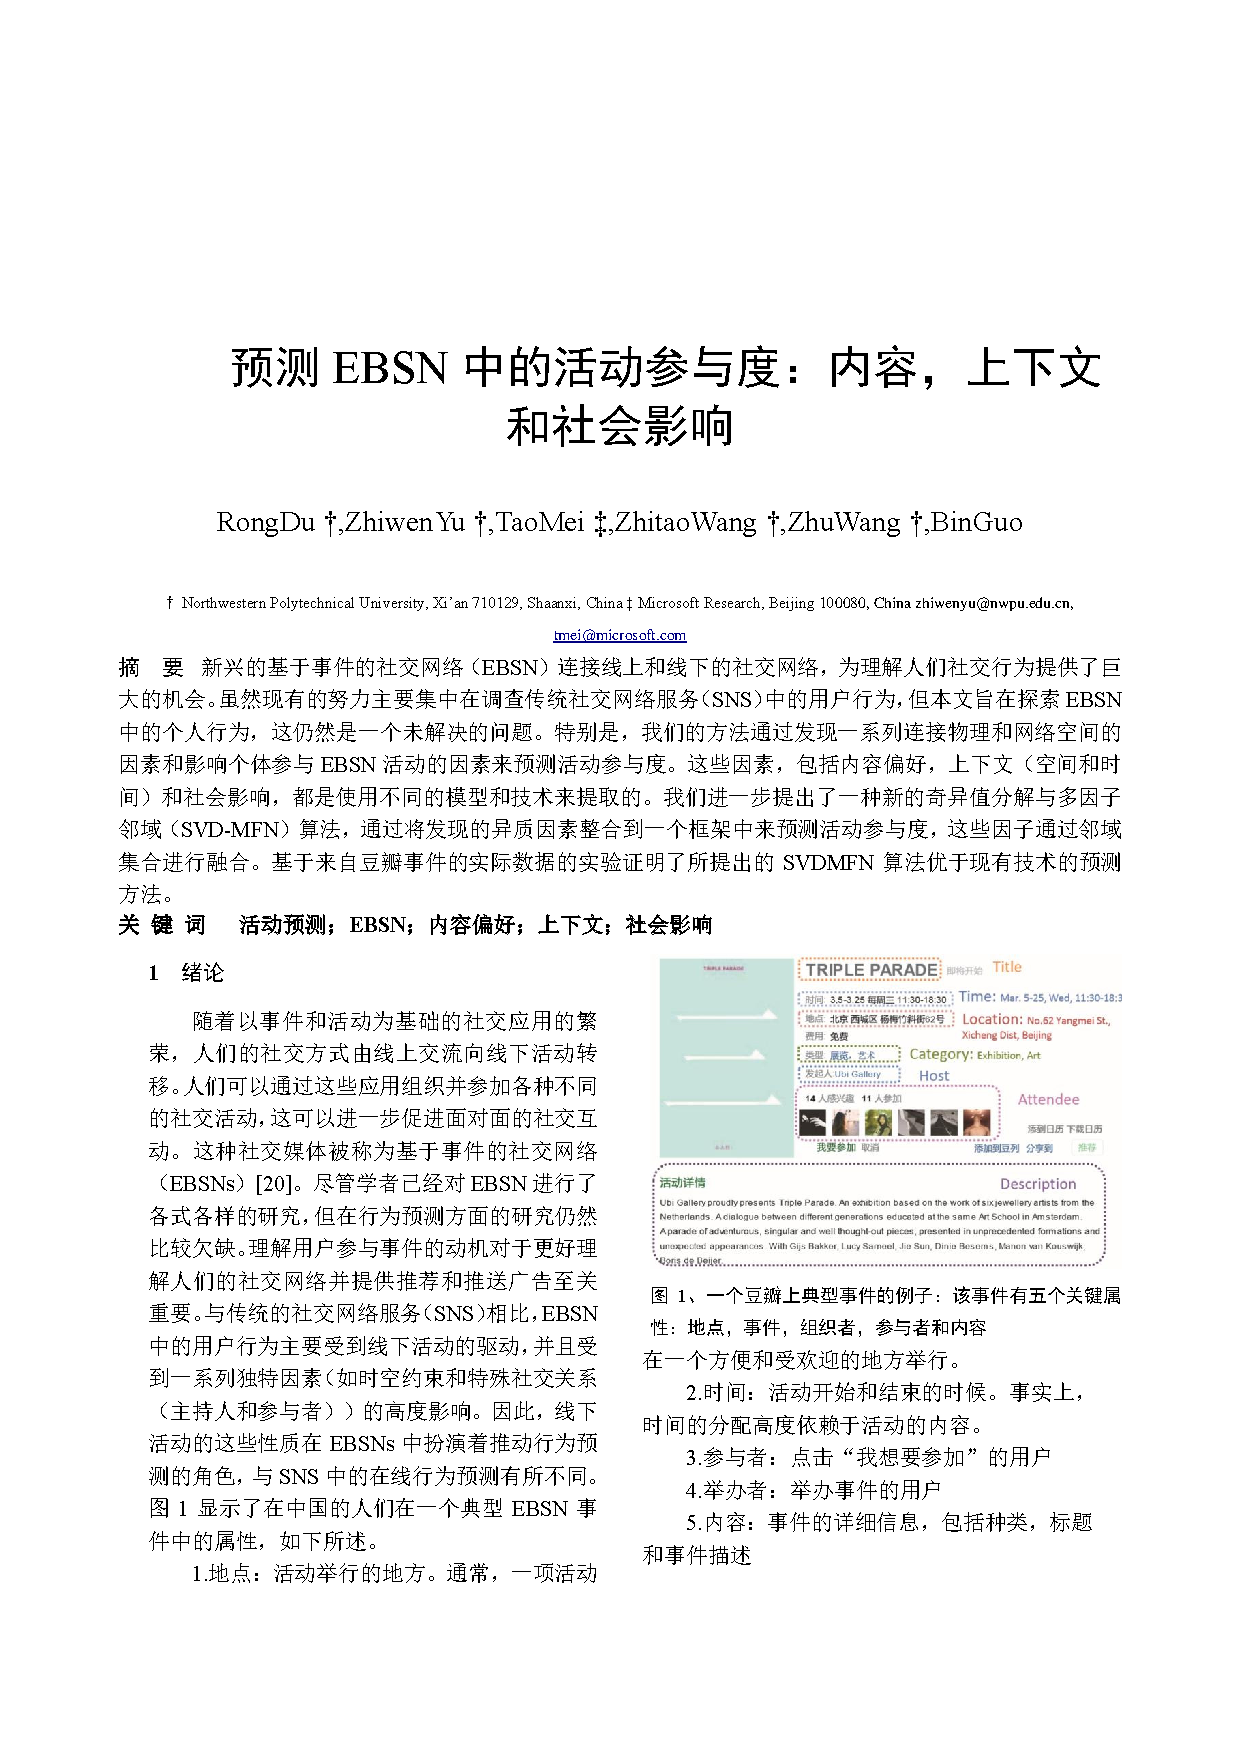
\includepdf[pages={1},pagecommand={\xjsection*{附~~录B 论文翻译译文}}]{translate.pdf}
\includepdf[pages={2-},pagecommand={\pagestyle{fancy}}]{translate.pdf}
% change odd to even
\includepdf[pages=-]{xuanti-0.pdf}
\includepdf[pages=-,landscape=true]{working_schedule-0.pdf}
\includepdf[pages=-]{midcheck-0.pdf}

\end{document}